%%%%%%%%%%%%%%%%%%%%%%%%%%%%%%%%%%%%%%%%%%%%%%%%%%%%%%%%%%%%%%%%%%%%%%%%%%%%%%%%
%Tutorial slides on Python.
%
% Author: FOSSEE 
% Copyright (c) 2009-2011, FOSSEE, IIT Bombay
%%%%%%%%%%%%%%%%%%%%%%%%%%%%%%%%%%%%%%%%%%%%%%%%%%%%%%%%%%%%%%%%%%%%%%%%%%%%%%%%

\documentclass[14pt,compress]{beamer}

% Modified from: generic-ornate-15min-45min.de.tex
\mode<presentation>
{
  \usetheme{Warsaw}
  \useoutertheme{infolines}
  \setbeamercovered{transparent}
}

\usepackage[english]{babel}
\usepackage[latin1]{inputenc}
%\usepackage{times}
\usepackage[T1]{fontenc}
\usepackage{pgf}

% Taken from Fernando's slides.
\usepackage{ae,aecompl}
\usepackage{mathpazo,courier,euler}
\usepackage[scaled=.95]{helvet}

\definecolor{darkgreen}{rgb}{0,0.5,0}

\usepackage{listings}
\lstset{language=Python,
    basicstyle=\ttfamily\bfseries,
    commentstyle=\color{red}\itshape,
  stringstyle=\color{darkgreen},
  showstringspaces=false,
  keywordstyle=\color{blue}\bfseries}

%%%%%%%%%%%%%%%%%%%%%%%%%%%%%%%%%%%%%%%%%%%%%%%%%%%%%%%%%%%%%%%%%%%%%%
% Macros
\setbeamercolor{emphbar}{bg=blue!20, fg=black}
\newcommand{\emphbar}[1]
{\begin{beamercolorbox}[rounded=true]{emphbar} 
      {#1}
 \end{beamercolorbox}
}
\newcounter{time}
\setcounter{time}{0}
\newcommand{\inctime}[1]{\addtocounter{time}{#1}{\tiny \thetime\ m}}

\newcommand{\typ}[1]{\lstinline{#1}}

\newcommand{\kwrd}[1]{ \texttt{\textbf{\color{blue}{#1}}}  }

%%% This is from Fernando's setup.
% \usepackage{color}
% \definecolor{orange}{cmyk}{0,0.4,0.8,0.2}
% % Use and configure listings package for nicely formatted code
% \usepackage{listings}
% \lstset{
%    language=Python,
%    basicstyle=\small\ttfamily,
%    commentstyle=\ttfamily\color{blue},
%    stringstyle=\ttfamily\color{orange},
%    showstringspaces=false,
%    breaklines=true,
%    postbreak = \space\dots
% }

%%%%%%%%%%%%%%%%%%%%%%%%%%%%%%%%%%%%%%%%%%%%%%%%%%%%%%%%%%%%%%%%%%%%%%
% Title page
\title[Advanced Sci Comp.]{Advanced Scientific Computing with
Python}
\subtitle{Introduction, NumPy and basic tools}

\author[FOSSEE group] {FOSSEE}

\institute[IIT Bombay] {Department of Aerospace Engineering\\IIT Bombay}
\date[] {PyCon Asia-Pacific,\\
Singapore\\
June 9, 2011
}
%%%%%%%%%%%%%%%%%%%%%%%%%%%%%%%%%%%%%%%%%%%%%%%%%%%%%%%%%%%%%%%%%%%%%%

%\pgfdeclareimage[height=0.75cm]{iitmlogo}{iitmlogo}
%\logo{\pgfuseimage{iitmlogo}}


%% Delete this, if you do not want the table of contents to pop up at
%% the beginning of each subsection:
\AtBeginSubsection[]
{
  \begin{frame}<beamer>
    \frametitle{Outline}
    \tableofcontents[currentsection,currentsubsection]
  \end{frame}
}

\AtBeginSection[]
{
  \begin{frame}<beamer>
    \frametitle{Outline}
    \tableofcontents[currentsection,currentsubsection]
  \end{frame}
}

% If you wish to uncover everything in a step-wise fashion, uncomment
% the following command: 
%\beamerdefaultoverlayspecification{<+->}

%%\includeonlyframes{current,current1,current2,current3,current4,current5,current6}

%%%%%%%%%%%%%%%%%%%%%%%%%%%%%%%%%%%%%%%%%%%%%%%%%%%%%%%%%%%%%%%%%%%%%%
% DOCUMENT STARTS
\begin{document}

\begin{frame}
  \maketitle
\end{frame}

%% \begin{frame}
%%   \frametitle{Outline}
%%   \tableofcontents
%%   % You might wish to add the option [pausesections]
%% \end{frame}

\begin{frame}
    \frametitle{Acknowledgement}
    \Large
    \begin{center}
        \alert{FOSSEE group (\url{fossee.in})} \\
        based at\\ 
        \alert{IIT Bombay}\\
        and funded by\\
        The National Mission on Education through ICT, \\
        \alert{Ministry of HRD, India}
    \end{center}
\end{frame}

\section{Checklist}
\begin{frame}
\frametitle{Checklist}
  \begin{enumerate}
    \item \alert{FIXME update when this session is done!}
    \item Data files: 
      \begin{itemize}
      \item \typ{anag.txt}
      \item \typ{holmes.txt}
      \item \typ{pendulum.txt}
      \item \typ{pos.txt}
      \item \typ{sslc1.txt}
      \end{itemize}
    \item Python scripts: 
      \begin{itemize}
      \item \typ{sslc_allreg.py}
      \item \typ{sslc_science.py}
      \end{itemize}
    \item Images
      \begin{itemize}
      \item \typ{lena.png}
      \item \typ{smoothing.gif}
      \end{itemize}
  \end{enumerate}
\end{frame}

\begin{frame}
  \frametitle{About the Tutorial}
  \begin{block}{Intended Audience}
  \begin{itemize}
       \item Engg., Mathematics and Science researchers with a
           good knowledge of Python, some OOP and knowledge of the material
           covered in the introductory tutorial.
  \end{itemize}
  \end{block}  

  \begin{block}{Goal: Successful participants will be able to}
    \begin{itemize}
      \item Start using Python as a tool for computational research

      \item Use some of the more advanced tools for their own research

    \end{itemize}
  \end{block}
\end{frame}

\section{Introduction}

\begin{frame}
    \frametitle{Tools available}
    \begin{itemize}
        \item IPython: the shell
        \item Numpy/Scipy: array and numerics
        \item Matplotlib/chaco: 2d plotting
        \item Mayavi: 3d plotting
        \item Enthought Tool Suite (ETS): application building
        \item Sympy: symbolic math 
        \item Cython: Python $\rightarrow$ C compiler 
        \item mpi4py, PyOpenCL, PyCUDA etc. 
            
            \vspace*{0.2in}
        \item Sage: very powerful symbolic and numeric tools
        \item Other specialized tools 

    \end{itemize}
\end{frame}

\section{IPython}

\begin{frame}
  \frametitle{IPython}
  \begin{itemize}
  \item Recommended interpreter, IPython:
    \url{http://ipython.scipy.org}
  \item Better than default Python shell
  \item Tab completion
  \item Easier object introspection
  \item Shell access!
  \item Command system
  \item Supports history and logging
  \item Embeddable
  \item Macros
  \item Custom interpreter
  \item Advanced features 
  \end{itemize}
\end{frame}

\begin{frame}[fragile]
  \frametitle{Basic IPython features}
  \begin{itemize}
  \item \verb+[--wthread|--gthread|--qthread]+
  \item \verb+--pylab+: Support for matplotlib
  \item \verb+object?+
  \item \verb+object??+
  \item \verb+%pdb+: pops up pdb on errors
  \item History: \texttt{<UpArrow>}
  \item Search: \texttt{<Ctrl-r> string}
  \item End of history: \texttt{Esc >}
  \item \verb+%run [options] file[.py]+
  \end{itemize}
\end{frame}

\begin{frame}[fragile]
  \frametitle{More IPython features}
  \begin{itemize}
  \item Input and output caching: \verb+In+, \verb+Out+
    \item \verb+%hist+ 
    \item Log the session using \verb+%logstart+, \verb+%logon+ and
    \verb+%logoff+
    \item \verb+%run -d:+ debug script with pdb
    \item \verb+%run -t+: time the script
    \item \verb+%run -p+: Profile the script
  \item \verb+%macro+ 
  \end{itemize}
\end{frame}

\begin{frame}[fragile]
  \frametitle{More IPython features \ldots}
  \begin{itemize}
  \item \verb+%edit [options] [args]+
  \item \verb+%cd, pushd, popd, dhist+ directory
    \item \verb+!command+: shell command
    \item \verb+files = %sx ls+ or \verb+files = !ls+
    \item \verb+%sx+ is quiet
    \item \verb+!ls $files+ passes the \verb+files+
    \item \verb+%alias alias_name cmd+
  \end{itemize}
\end{frame}

\begin{frame}[fragile]
  \frametitle{More IPython features \ldots}
  \begin{itemize}
  \item \verb+;+ suppresses output
  \item \verb+%bookmark+
  \item \verb+%who, %whos+: print information on variables
  \item \verb+%save+: save lines to a file
  \item \verb+%time statement+
  \item \verb+%timeit statement+
  \item Profiles: \verb+math, scipy, numeric, pysh+ etc.
  \item \verb+%magic+: \alert{Show help on all magics}
  \end{itemize}
\end{frame}

\section{NumPy arrays}

\newcommand{\num}{\texttt{numpy}}


\begin{frame}[fragile]
  \frametitle{The \num\ module}
    \begin{itemize}
        \item \alert{Mostly a recap}
    \item Efficient, powerful array type
    \item Abstracts out standard operations on arrays
    \item COnvenience functions
    \item \typ{ipython --pylab} imports part of numpy
    \item Without the Pylab mode do:
    \end{itemize}
    \begin{lstlisting}
In []: import numpy

In []: from numpy import *
    \end{lstlisting}
\end{frame}

\begin{frame}
  \frametitle{\num\ arrays}
  \begin{itemize}
  \item Fixed size (\typ{arr.size})
  \item Same type (\typ{arr.dtype})
  \item Arbitrary dimensionality: \typ{arr.shape}
  \item \typ{shape}: extent (size) along each dimension
  \item \typ{arr.itemsize}: number of bytes per element
  \item \alert{Note:} \typ{shape} can change so long as the \typ{size}
      is constant
  \item Indices start from 0
  \item Negative indices do the right thing.
  \end{itemize}
\end{frame}

\begin{frame}[fragile]
  \frametitle{\num\ arrays}
\begin{lstlisting}
In []: a = array([1,2,3,4])
In []: b = array([2,3,4,5])

In []: print a[0], a[-1]
1, 4

In []: a[0] = -1
In []: a[0] = 1
\end{lstlisting}
Operations are elementwise
\end{frame}

\begin{frame}[fragile]
  \frametitle{Simple operations}
\begin{lstlisting}
In []: a + b  
Out[]: array([3, 5, 7, 9])
In []: a*b
Out[]: array([2, 6, 12, 20])
In []: a/b
Out[]: array([0, 0, 0, 0])
\end{lstlisting}
Operations are elementwise, types matter.
\end{frame}

\begin{frame}[fragile]
  \frametitle{Examples}
\noindent \typ{pi} and \typ{e} are defined.
\begin{lstlisting}
In []: x = linspace(0.0, 10.0, 200)
In []: x *= 2*pi/10
# apply functions to array.
In []: y = sin(x)
In []: y = cos(x)
In []: x[0] = -1
In []: print x[0], x[-1]
-1.0 10.0
\end{lstlisting}
\end{frame}

\begin{frame}[fragile]
    \frametitle{\typ{size, shape, rank} etc.}
\vspace*{-8pt}
\begin{lstlisting}
In []: x = array([1., 2, 3, 4])
In []: size(x)
Out[]: 4
In []: x.dtype
dtype('float64')
In []: x.shape
Out[] (4,)
In []: rank(x)
Out[]: 1
In []: x.itemsize
Out[]: 8
\end{lstlisting}
\end{frame}


\begin{frame}[fragile]
  \frametitle{Multi-dimensional arrays}
\begin{lstlisting}
In []: a = array([[ 0, 1, 2, 3],
  ...:            [10,11,12,13]])
In []: a.shape # (rows, columns)
Out[]: (2, 4)

In []: a[1,3] 
Out[]: 13

In []: a[1,3] = -1
In []: a[1] # The second row
array([10,11,12,-1])
In []: a[1] = 0 # Entire row to zero.
\end{lstlisting}

\end{frame}

\begin{frame}[fragile]
  \frametitle{Slicing arrays}
  \vspace*{-0.2in}
\begin{lstlisting}
In []: a = array([[1,2,3], [4,5,6], 
  ...:            [7,8,9]])
In []: a[0,1:3]
Out[]: array([2, 3])
In []: a[1:,1:]
Out[]: array([[5, 6],
              [8, 9]])
In []: a[:,2]
Out[]: array([3, 6, 9])
In []: a[0::2,0::2] # Striding...
Out[]: array([[1, 3],
              [7, 9]])
# Slices refer to the same memory!
\end{lstlisting}
\end{frame}

\begin{frame}[fragile]
  \frametitle{Array creation functions}
  \begin{itemize}
  \item \typ{array(object)}
  \item \typ{arange([start,] stop, [step])}
  \item \typ{linspace(start, stop, num=50)}
  \item \typ{ones(shape)}
  \item \typ{zeros((d1,...,dn))}
  \item \typ{empty((d1,...,dn))}
  \item \typ{identity(n)}
  \item \typ{ones\_like(x)}, \typ{zeros\_like(x)}, \typ{empty\_like(x)}
  \end{itemize}
  May pass an optional \typ{dtype=} keyword argument

  For more dtypes see: \typ{numpy.typeDict}
\end{frame}

\begin{frame}[fragile]
  \frametitle{Creation examples}
  \vspace*{-0.25in}
\begin{lstlisting}
In []: a = array([1,2,3], dtype=float)
In []: ones( (2, 3) )
Out[]: array([[ 1.,  1.,  1.],
              [ 1.,  1.,  1.]])
In []: identity(3)
Out[]: array([[ 1.,  0.,  0.],
              [ 0.,  1.,  0.],
              [ 0.,  0.,  1.]])
In []: ones_like(a)
Out[]: array([ 1.,  1.,  1.,  1.])
\end{lstlisting}
\end{frame}

\begin{frame}[fragile]
  \frametitle{Array math}
  \begin{itemize}
  \item Basic \alert{elementwise} math (given two arrays \typ{a, b}):
    \begin{itemize}
        \item \typ{a + b} $\rightarrow$ \typ{add(a, b)} 
        \item \typ{a - b}, $\rightarrow$ \typ{subtract(a, b)} 
        \item \typ{a * b}, $\rightarrow$ \typ{multiply(a, b)} 
        \item \typ{a / b}, $\rightarrow$ \typ{divide(a, b)} 
        \item \typ{a \% b}, $\rightarrow$ \typ{remainder(a, b)} 
        \item \typ{a ** b}, $\rightarrow$ \typ{power(a, b)}
    \end{itemize}
  \item Inplace operators: \typ{a += b}, or \typ{add(a, b,
      a)}
  \item Logical operations: \typ{==, !=, <, >}, etc.
  \item \typ{sin(x), arcsin(x), sinh(x)},
      \typ{exp(x), sqrt(x)} etc.
  \item \typ{sum(x, axis=0), product(x, axis=0)}
  \item \typ{dot(a, b)}
  \end{itemize}
\end{frame}

\section{Advanced Numpy}

\begin{frame}[fragile]
  \frametitle{Special indexing}
  \begin{lstlisting}
In []: a = arange(9)**2
In []: a
Out[]: array([ 0, 1, 4, ... 49, 64])

# Access only some indices!
In []: a[ [1, 5, 2, -3] ]
Out[]: array([ 1, 25,  4, 36])

# Assignment.
In []: a[ [1, 5, 2, -3] ] = -1
In []: a[ [1, 5, 2, -3] ] = [1,25,4,36]
  \end{lstlisting}
\end{frame}

\begin{frame}[fragile]
  \frametitle{Special indexing}
  \begin{lstlisting}
In []: a.shape = 3,3

In []: a[ [0, 2] ] # The rows
Out[]: array([[ 0,  1,  4],
              [36, 49, 64]])
# Specific elements
In []: a[ [ [0,1], [2,0] ] ]
Out[]: array([4, 9])

In []: a[ [0,1], [2,0] ] 
Out[]: array([4, 9])

  \end{lstlisting}
\end{frame}

\begin{frame}[fragile]
  \frametitle{Boolean indices}
  \begin{lstlisting}
In []: a > 5
Out[]: 
array([[False, False, False],
       [ True,  True,  True],
       [ True,  True,  True]], dtype=bool)

In []: a[a>5] = -1
In []: a
Out[]: 
array([[ 0,  1,  4],
       [-1, -1, -1],
       [-1, -1, -1]])
  \end{lstlisting}
\end{frame}


\begin{frame}[fragile]
  \frametitle{Broadcasting}
  \begin{lstlisting}
In []: a = arange(4)
In []: b = arange(5)
In []: a+b #Does this work?
In []: a+3
In []: c = array([3])
In []: a+c #Works!
In []: b+c #But how?
In []: a.shape, b.shape, c.shape
  \end{lstlisting}
  \begin{itemize}
    \item Enter Broadcasting!
  \end{itemize}
\end{frame}

\begin{frame}[fragile]
  \frametitle{Broadcasting}
  \begin{columns}
    \column{0.65\textwidth}
    \hspace*{-1.5in}
    \begin{lstlisting}
      In []: a = arange(4)
      In []: a+3
      array([3, 4, 5, 6])
    \end{lstlisting}
    \column{0.35\textwidth}
    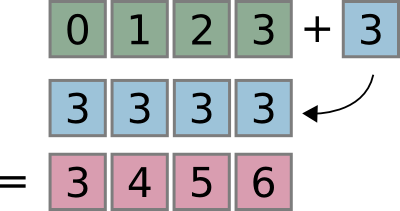
\includegraphics[height=0.7in, interpolate=true]{data/broadcast_scalar}
  \end{columns}
\end{frame}

\begin{frame}[fragile]
  \frametitle{Broadcasting in 3D}
    \begin{lstlisting}
      In []: x = ones((3, 5, 1))
      In []: y = ones(8)
      In []: (x + y).shape
      (3, 5, 8)
    \end{lstlisting}
    \begin{figure}
      \begin{center}
      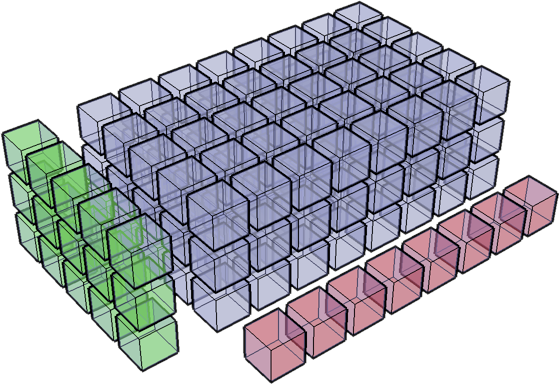
\includegraphics[height=1.5in, interpolate=true]{data/array_3x5x8}        
      \end{center}
    \end{figure}
\end{frame}

\begin{frame}[fragile]
  \frametitle{Copies \& Views}
  \vspace{-0.1in}
  \begin{lstlisting}
    In []: a = arange(1,9); a.shape=3,3
    In []: b = a
    In []: b is a
    In []: b[0,0]=0; print a
    In []: c = a.view()
    In []: c is a
    In []: c.base is a
    In []: c.flags.owndata
    In []: d = a.copy()
    In []: d.base is a
    In []: d.flags.owndata
  \end{lstlisting}
\end{frame}

\begin{frame}[fragile]
  \frametitle{Copies \& Views}
  \vspace{-0.1in}
  \begin{lstlisting}
    In []: b = a[0,1:3]
    In []: c = a[0::2,0::2]
    In []: a.flags.owndata
    In []: b.flags.owndata
    In []: b.base
    In []: c.base is a
  \end{lstlisting}
  \begin{itemize}
  \item Slicing and Striding just reference the same memory
  \item They produce views of the data, not copies
  \end{itemize}
\end{frame}

\begin{frame}[fragile]
  \frametitle{Copies contd \ldots}
  \begin{lstlisting}
    In []: a = arange(1, 10, 2)
    In []: b = a[array([0,2,3])]
    In []: b.flags.owndata
    In []: abool=a>5
    In []: c = a[abool]
    In []: c.flags.owndata
  \end{lstlisting}
  \begin{itemize}
  \item Indexing arrays or Boolean arrays produce copies
  \end{itemize}
%\inctime{15}
\end{frame}


\begin{frame}[fragile]
  \frametitle{An exercise}

Plot the mandelbrot set. 

Consider points in the complex plane.  For each point, $c$, calculate
$z_{n+1} = z_n^2 + c$, with $z_0 = 0$.  Note that if $z_i > 2$ the
solution will diverge.  We would like to plot the number of iterations a
point diverges in.

Given \typ{w, h} as width and height of image.  Region of interest is
[-2, -1.4] to [0.8, 1.4].

%x, y = mgrid[ -2:0.8:w*1j, -1.4:1.4:h*1j ]

\end{frame}

\begin{frame}[fragile]
  \frametitle{Naive solution}
  \begin{lstlisting}
      # Naive solution here.
  \end{lstlisting}
\end{frame}

\begin{frame}[fragile,allowframebreaks]
  \frametitle{Numpy solution}
  \small
  \begin{lstlisting}
      # Numpy solution here.
from numpy import *
import pylab

def mandelbrot( h,w, maxit=20 ):
    '''Returns an image of the Mandelbrot fractal of size (h,w).
    '''
    y,x = ogrid[ -1.4:1.4:h*1j, -2:0.8:w*1j ]
    c = x+y*1j
    z = c
    divtime = maxit + zeros(z.shape, dtype=int)

    for i in xrange(maxit):
            z  = z**2 + c
            diverge = z*conj(z) > 2**2            # who is diverging
            div_now = diverge & (divtime==maxit)  # who is diverging now
            divtime[div_now] = i                  # note when
            z[diverge] = 2                        # avoid diverging too much

    return divtime

pylab.imshow(mandelbrot(400,400))
pylab.show()
  \end{lstlisting}
\end{frame}


\begin{frame}[fragile]
    \frametitle{Record arrays}
    \begin{itemize}
        \item Numpy arrays
        \item Allow field access 
    \end{itemize}
    \begin{lstlisting}
In []: typ = [('id', int), ('x', float)]
In []: rec = numpy.zeros(10, dtype=typ)
In []: rec['id'] = range(10)
In []: rec['x'] = random.random(size=10)
    \end{lstlisting}
    \begin{itemize}
        \item Data type can be any valid numpy dtype
        \item Very convenient
    \end{itemize}
\end{frame}

\begin{frame}[fragile]
    \frametitle{Record array views}
Can obtain easier attribute access:

    \begin{lstlisting}
In []: ra = rec.view(recarray)
In []: print ra.id, ra.x
    \end{lstlisting}
\end{frame}

\begin{frame}[fragile]
    \frametitle{\typ{csv2rec}}
    \begin{itemize}
        \item CSV file $\rightarrow$ Record array
        \item Very convenient and powerful
        \item Automatic naming
        \item Handles missing data
        \item Handles different delimiters
    \end{itemize}
    \begin{lstlisting}
In []: csv2rec?
    \end{lstlisting}
\end{frame}

\begin{frame}[fragile]
    \frametitle{\typ{csv2rec} example data}
    \begin{itemize}
        \item Describe the data here
    \end{itemize}
\end{frame}

\begin{frame}[fragile]
    \frametitle{\typ{csv2rec} example}
    \begin{lstlisting}
In []: data = csv2rec('data.csv')
In []: scatter(data['x'], data['y'], 
  ...:         c=data['value'])
    \end{lstlisting}
\end{frame}


\section{SciPy}
\begin{frame}[plain]
  \frametitle{SciPy}
  \begin{itemize}
  \item Provides:
    \begin{itemize}
    \item Linear algebra
    \item Numerical integration
    \item Fourier transforms
    \item Signal processing
    \item Special functions
    \item Statistics
    \item Optimization
    \item Image processing
    \item ODE solvers
    \end{itemize}
  \item Uses LAPACK, QUADPACK, ODEPACK, FFTPACK etc. from netlib
  \end{itemize}
\end{frame}



\begin{frame}[fragile,plain]
  \frametitle{Matplotlib plots}
  \begin{columns}
    \column{0.5\textwidth}
    \hspace*{-0.5in}
    \pgfimage[height=2in, interpolate=true]{../MEDIA/python/xyplot}
    \column{0.45\textwidth}
    \begin{block}{Example code}
    \tiny
\begin{lstlisting}
t1 = arange(0.0, 5.0, 0.1)
t2 = arange(0.0, 5.0, 0.02)
t3 = arange(0.0, 2.0, 0.01)
subplot(211)
plot(t1, cos(2*pi*t1)*exp(-t1), 'bo', 
     t2, cos(2*pi*t2)*exp(-t2), 'k')
grid(True)
title('A tale of 2 subplots')
ylabel('Damped')
subplot(212)
plot(t3, cos(2*pi*t3), 'r--')
grid(True)
xlabel('time (s)')
ylabel('Undamped')
\end{lstlisting}
    \end{block}
  \end{columns}
\end{frame}

\begin{frame}[plain]
    \begin{center}
  \pgfimage[height=1.5in, interpolate=true]{../MEDIA/python/errorbar}  
  \pgfimage[height=1.5in, interpolate=true]{../MEDIA/python/log}  
    \end{center}
\end{frame}
\begin{frame}[plain]
    \begin{center}
  \pgfimage[height=1.75in, interpolate=true]{../MEDIA/python/barchart}  
  \pgfimage[height=1.75in, interpolate=true]{../MEDIA/python/piechart}  
    \end{center}
\end{frame}

\begin{frame}[plain]
    \begin{center}
  \pgfimage[height=1.75in, interpolate=true]{../MEDIA/python/scatter}  
  \pgfimage[height=1.75in, interpolate=true]{../MEDIA/python/histogram}  
    \end{center}
\end{frame}

\begin{frame}[plain]
    \begin{center}
  \pgfimage[height=2in, interpolate=true]{../MEDIA/python/polar}  
  \pgfimage[height=1.75in, interpolate=true]{../MEDIA/python/quiver}  
    \end{center}
\end{frame}
\begin{frame}[plain]
    \begin{center}
  \pgfimage[height=2.5in, interpolate=true]{../MEDIA/python/plotmap}  
    \end{center}
\end{frame}

\begin{frame}[plain]
    \frametitle{IPython + SciPy + Matplotlib}
  \begin{center}
  \pgfimage[height=1.75in, interpolate=true]{../MEDIA/python/contour}  
  \pgfimage[height=2.75in, interpolate=true]{../MEDIA/python/scipy_screenie}  
  \end{center}
\end{frame}

\end{document}

